
\chapter{非次模影响力传播模型}
上一章介绍了影响力最大化问题的发展情况和现有算法。
但是这些算法都是基于次模的影响力传播模型,而且在设计算法的过程中大多也利用了次模的性质。
在本章,我们会介绍非次模模型,本文的研究也是基于所提出的非次模模型。

\section{$\varepsilon$-次模逼近函数}
通用阈值模型是影响力最大化问题中最重要的模型之一。
通常情况下,我们关注阈值函数(threshold function)的两个性质——次模性质(submodularity)和超模性质(supermodularity)。
次模性质可以被理解为在向种子集合添加新节点时,现有种子集合越大,获得的收益越小,也就是边际收益递减。
与之相反,超模性质是边际效益递增。
对于通用阈值模型来说,阈值函数的次模性质是贪心算法近似比的保证\cite{Mossel2007sub},
在这篇论文里,我们想要研究阈值函数是近次模函数的模型,这个函数被定义为$\varepsilon$-次模逼近函数($\varepsilon$-almost submodular function)。
接下来我们给出次模,超模和$\varepsilon$-次模逼近函数的精确定义。

\begin{definition}[次模 (Submodular)]
对于一个定义在集合上的函数$f:2^V \to \mathbb{R}$,
如果对于$V$的任意子集$S \subseteq T \subseteq V$和点$v \not\in T$都有
$f(S \cup \{v\}) - f(S) \geq f(T \cup \{v\}) - f(T)$,
则称$f$为次模函数。
\end{definition}

\begin{definition}[超模 (Supermodular)]
对于一个定义在集合上的函数$f:2^V \to \mathbb{R}$,
如果对于$V$的任意子集$S \subseteq T \subseteq V$和点$v \not\in T$都有
$f(S \cup \{v\}) - f(S) \leq f(T \cup \{v\}) - f(T)$,
则称$f$为次模函数。
\end{definition}

\begin{definition}[$\varepsilon$-次模逼近 ($\varepsilon$-Almost Submodular)]
对于一个定义在集合上的函数$f:2^V \to \mathbb{R}$,
如果存在一个同样定义在$2^V$上的次模函数$f^{sub}$和一个正数$\varepsilon<1$,
对于任意的$S \subseteq V$都有$f^{sub}(S) \geq f(S) \geq (1-\varepsilon)f^{sub}(S)$,
则称$f$为$\varepsilon$-次模逼近函数。
$f$的次模上届和下届函数分别是$\overline{f}$和$\underline{f}$。
\end{definition}

本文只讨论有向图上的影响力传播,对于阈值函数$f$,如果函数值只依赖于输入集合的大小,我们可以简写为$f_v(S) = f_v(|S|)$。
$\varepsilon$-次模逼近函数描述了一类很接近次模但又不是次模的函数,直观上看$\varepsilon$-次模逼近函数的性质会和次模函数很接近。
本文主要研究非次模问题,在后续章节以$\varepsilon$-次模逼近函数为切入口,会讨论在阈值函数为$\varepsilon$-次模逼近函数时,影响力最大化问题能能否被近似。
$\varepsilon$-次模逼近函数在现实生活中也是有意义的,现实网络中很多影响传播过程都被观测到有非次模的现象。
Backstrom\cite{backstrom2006group}等人研究了LiveJounral和DBLP两个大型的社交网络数据,
他们把用户加入LiveJounral社区的概率看作已经加入社区用户的数量的函数,并在论文的Figure 1中绘制了该函数,如图\ref{fig:LiveJounral}所示,
者可以看做用户的阈值函数。
可以看到函数的整体走势图是上凸的,图中的$k$就是输入集合大小。但是在$k=1$时,函数值有一个轻微的下移,所以函数整体上是次模的,但是在输入集合较小时不满足。
\begin{figure}[h]
	\centering
	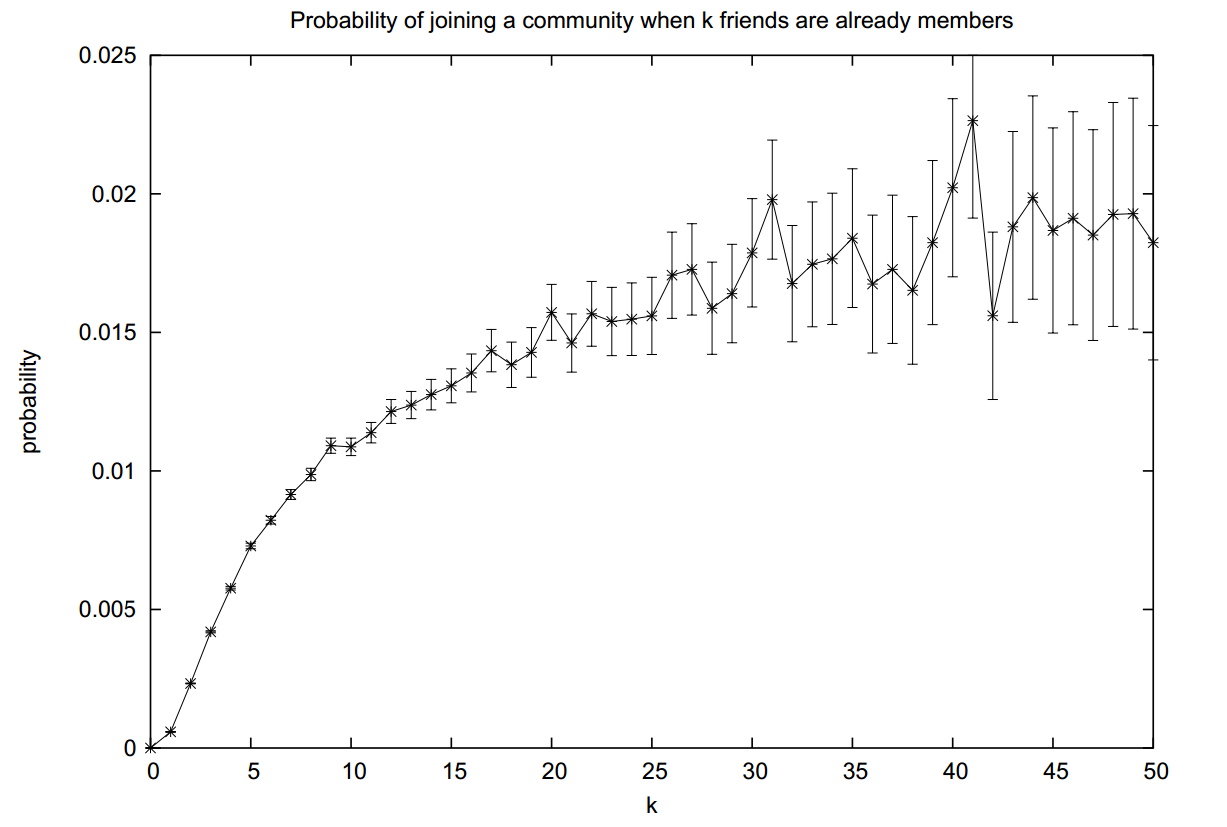
\includegraphics[width=0.8\textwidth]{LiveJounral.png}
	\caption{LiveJounral社区\cite{backstrom2006group}}\label{fig:LiveJounral}
\end{figure}
此外,杨洋\cite{yang2016role}等人观测了Flickr网络的情绪传播,把用户变开心的概率看做开心朋友数量的函数,
绘制的图片见原论文Figure 1(a),这里展示为图\ref{fig:Flickr}。
从图中可以看出整体上用户被影响的概率和朋友数量是一个超线性关系,也就是超模性质。
不同的用户阈值函数也不同,对于领导来说,阈值函数更偏向超模,而对普通用户阈值函数是次模的。
我们在后续的实验中也会采用这两种类似的$\varepsilon$-次模逼近函数设定。
\begin{figure}[h]
	\centering
	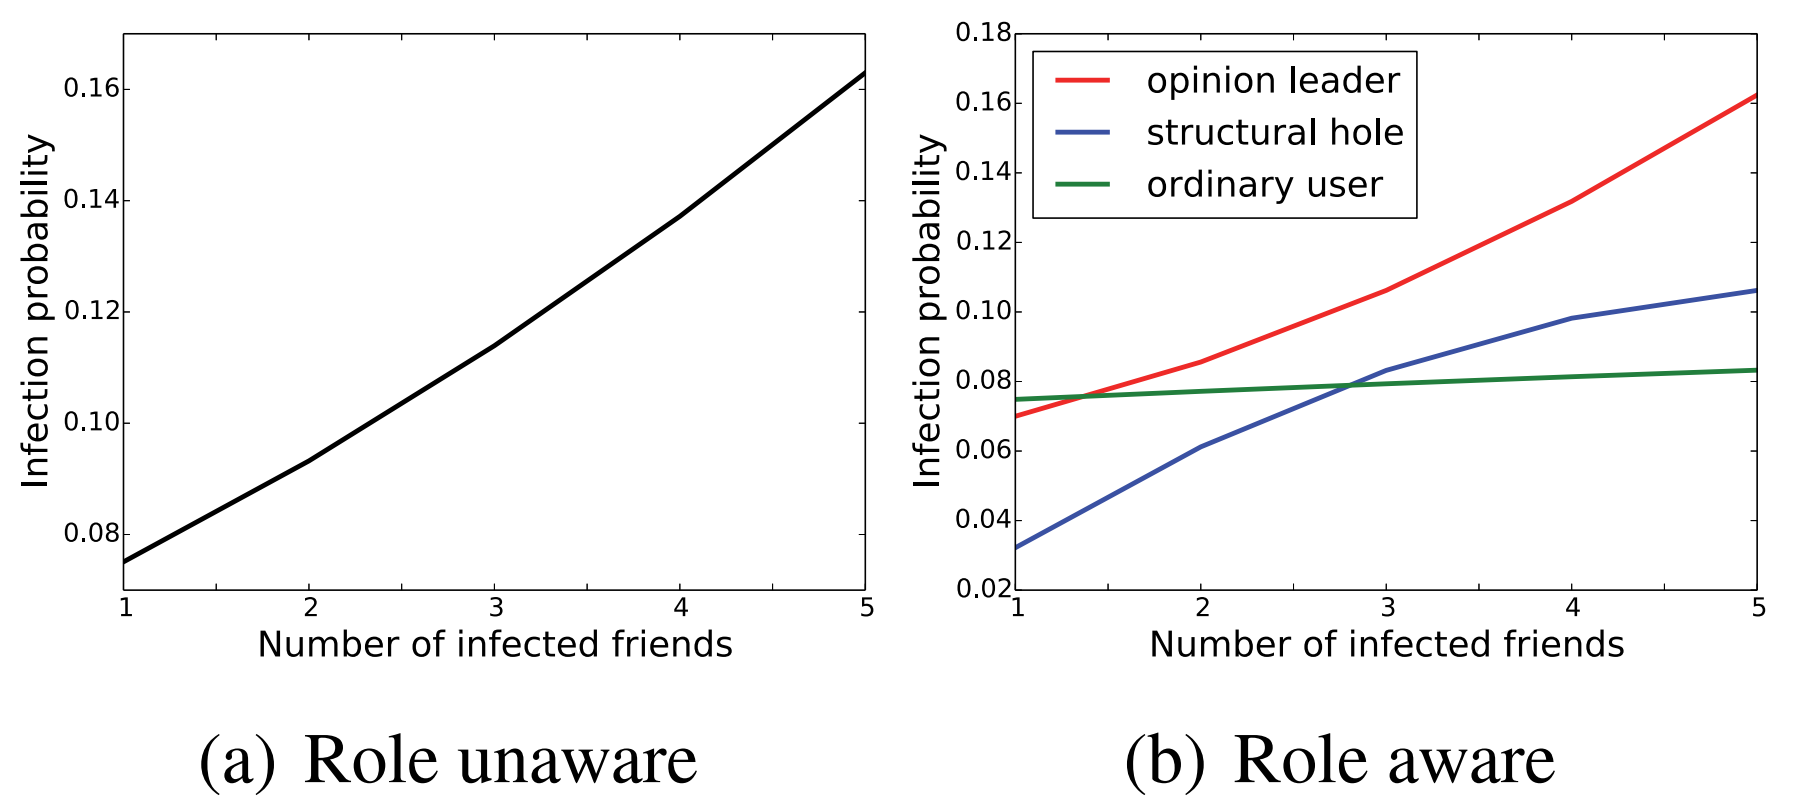
\includegraphics[width=0.8\textwidth]{Flickr.png}
	\caption{Flickr社区\cite{yang2016role}}\label{fig:Flickr}
\end{figure}

在给定$\varepsilon$-次模逼近函数定义和动机之后,我们介绍本文主要研究的问题。
本文主要研究图中有部分节点的阈值函数是$\varepsilon$-次模逼近函数的情况。
\begin{definition}[$(\gamma,\varepsilon)$-次模逼近图 ($(\gamma,\varepsilon)$-Almost Submodular Graph)]
给定参数$\gamma, \varepsilon \in (0,1)$,
一个$n$个节点的图如果至多有$n^{\gamma}$个节点阈值函数是$\varepsilon$-次模逼近,其余节点的阈值函数是次模的,
我们称其为是{\it $(\gamma,\varepsilon)$-次模逼近图}或者{\it $(\gamma,\varepsilon)$-次模逼近网络}。
\end{definition}
后续为了简便,阈值函数是$\varepsilon$-次模逼近的节点简写为{\it $\varepsilon$-次模逼近节点},
阈值函数是模的节点简写为{\it 次模节点},
$\varepsilon$-次模逼近可写作{\it $\varepsilon$-AS},
包含$\varepsilon$-次模逼近节点的图可写作{\it $\varepsilon$-次模逼近网络}。
$\gamma, \varepsilon$描述了图偏离次模的程度,$\gamma, \varepsilon$越大,图上影响力函数偏离次模越远。
接着,我们定义$(\gamma,\varepsilon)$-次模逼近图上的影响力最大化问题$(\gamma,\varepsilon)$-ASIM,也是本文研究的重点。

\begin{definition}[$(\gamma,\varepsilon)$-次模影响力最大化 ($(\gamma,\varepsilon)$-ASIM)]
给定一个$(\gamma,\varepsilon)$-次模逼近图和输入$k$,$(\gamma,\varepsilon)$-次模影响力最大化问题是
在这个有$n^{\gamma}$个$\varepsilon$-次模逼近节点节点的图上寻找影响力最大的,大小不超过$k$的种子集合。
\end{definition}


\section{$k$-激活函数}
接下来本节介绍$k$-激活函数。

\subsection{传染病模型}
$k$-激活本质上是用{\it 传染病}去模拟信息、疾病和想法在网络中的扩散。
网络中的节点都有三种状态:{\it 未激活}(inactive)、{\it 暴露}(exposed)和{\it 已激活}(activated)。
节点可以从未激活状态转变为状态,然后再进入激活状态,但是不能反方向转变,例如不能从已激活的状态变成未激活状态。

传染病传染的过程可以用离散的时间步骤$0,1,2,\ldots$来描述。
如果一个节点$u$在$t-1$时间有至少$k$个已经感染的邻居节点
(在有向图中指有$k$个已感染节点发出的有向边指向$u$),
那么在时间$t\ge 1$节点$u$就变为暴露状态,$k$是传染病的阈值。
一个已经暴露的节点可以立即或者在后续时间步骤中转变为感染状态,
这取决于传染病扩散的方式。
{\it 简单传染病}指$k=1$的传染病,也就是说$u$的一个已感染的邻居就可以让$u$变为感染状态(有可能感染$u$)。
而{\it 复杂传染病}则较难传染,因为复杂传染病的阈值$k \geq 2$,要感染一个新的节点,
至少需要两个已感染的邻居节点。
阈值$k\ge 2$的传染病称为$k$-复杂传染病。

对于$k$-复杂传染病来说,对应的阈值函数恰好是$k$-激活函数,$k$-激活函数的定义如下
\begin{definition}[$k$-激活]
对于一个定义在集合上的函数$f:2^V \to \mathbb{R}$,
如果对于$V$的任意元素个数小于$k$的子集$S \subseteq V:|S|<k$都有$f(S) = 0$,
并且任意元素个数不小于$k$的子集$S \subseteq V:|S|\geq k$都有$f(S) = 1$,
则称$f$为$k$-激活函数。
\end{definition}


本文主要研究传染病多快把整个网络都传染,这个可以用{\it 传播时间}来描述,
而在网络中的强连接和弱连接都固定后传播时间是定值。
传播时间是指从$k$个种子节点开始,整个网络都被感染时经过的时间步数。

\subsection{传染病模型下的路由}

本文主要研究了一种比较像分散式路由\cite{Kleinberg2000small}的扩散方式,
我们称之为{\it $k$-复杂传染病的路由}(简称{\it 复杂路由}),也称为{\it $k$-激活路由}。

在复杂路由中,最初会选择一个节点$t$作为目标,同时也有$k$个种子节点。
复杂路由的任务是尽快激活目标节点$t$,不同于传播过程的是,
每一个时间步骤中所有被暴露的节点不会被立即感染。
每一步,我们只能从暴露状态的节点集合中选择一个节点来感染。
选择节点的策略称为路由策略。
更进一步,当在时间$i$选择了节点$u$去感染时,算法仅仅知道已感染节点集合的所有邻居(在有向图中是已感染节点发出的有向边指向的节点)。
复杂路由在日常生活中的情景比较像一群人想要去影响一个目标,
但是无法直接影响到目标。
于是这群人逐渐的扩大自己的势力,拉拢他们认为可以对劝说目标有帮助的人入伙,最终影响到目标。
在扩大势力的时候,他们只知道已经入伙的人的朋友,而且拉拢入伙需要一定的代价,在每一步只能选择拉拢一个人。
注意到如果把$k$设置为$1$,
并且要求下一个被激活的节点是最新激活节点的邻居,这就是Kleinberg研究的分散式路由\cite{Kleinberg2000small}。

为了研究路由找到目标的速度,本文定义{\it $k$-激活路由时间}
为通过$k$-激活路由方式激活距离种子节点曼哈顿距离最远的目标节点$t$所需要的步骤。


\section{本章小结}
本章主要介绍了本文后续降采用的阈值函数和相关问题定义
3.1节介绍了$\varepsilon$-次模逼近函数和函数在现实生活中的意义,定义了$(\gamma,\varepsilon)$-次模影响力最大化问题。
3.2节介绍了$k$-激活函数和对应的复杂传染病模型,同时提供了离散路由的定义。